\documentclass[12pt]{article}

% Use packages %
\usepackage{graphicx, courier, amsmath, amssymb, amscd, amsfonts, mathtools, bm, esint, leftidx, extarrows, latexsym, relsize, color, tikz, comment}
\usepackage[obeyspaces]{url}% http://ctan.org/pkg/url

% Set length %
\setlength{\textwidth}{160mm}
\setlength{\textheight}{235mm}
\setlength{\oddsidemargin}{-0mm}
\setlength{\topmargin}{-10mm}

% Define h-bar %
\newsavebox{\myhbar}
\savebox{\myhbar}{$\hbar$}
\renewcommand*{\hbar}{\mathalpha{\usebox{\myhbar}}}

% Chinese input %
%\usepackage{xeCJK} 
%\setCJKmainfont{微軟正黑體}
%\usepackage[T1]{fontenc}
%\makeatletter

% Equation number %
%\@addtoreset{equation}{section} 
%\renewcommand\theequation{{\thesection}.{\arabic{equation}}}
%\makeatletter 

% Helper Command %
\newcommand{\argmin}{\operatornamewithlimits{argmin}}
\newcommand{\rmnum}[1]{\romannumeral #1} 
\newcommand{\Rmnum}[1]{\expandafter\@slowromancap\romannumeral #1@}
\newcommand{\overbar}[1]{\mkern 1.5mu\overline{\mkern-1.5mu#1\mkern-1.5mu}\mkern 1.5mu}
\makeatother
\newcommand*{\QEDA}{\hfill\ensuremath{\blacksquare}}
\newcommand*{\QEDB}{\hfill\ensuremath{\square}}
\newcommand*{\BmVert}{\bigm\vert}
\newcommand{\bigslant}[2]{{\raisebox{.2em}{$#1$}\left/\raisebox{-.2em}{$#2$}\right.}}
\newcommand{\Nelements}[3]{\left\{ #1, ~ #2, \ldots, ~ #3 \right\}}
\newcommand{\CBrackets}[1]{\left\{#1\right\}}
\newcommand{\SBrackets}[1]{\left[#1\right]}
\newcommand{\ParTh}[1]{\left(#1\right)}
\newcommand{\Ceil}[1]{\left\lceil#1\right\rceil}
\newcommand{\Floor}[1]{\left\lfloor#1\right\rfloor}
\newcommand{\BF}[1]{{\bf#1}}
\newcommand{\Inverse}[1]{{#1}^{-1}}
\newcommand{\Generator}[1]{\left\langle#1\right\rangle}
\newcommand{\AbsVal}[1]{\left|#1\right|}
\newcommand{\VecAbsVal}[1]{\left\|#1\right\|}
\newcommand{\BSlash}[2]{\left.#1\middle\backslash#2\right.}
\newcommand{\Divide}[2]{\left.#1\middle/#2\right.}
\newcommand{\SciNum}[2]{#1\times{10}^{#2}}
\newcommand{\Matrix}[2]{\ParTh{\begin{array}{#1}#2\end{array}}}
\newcommand{\MatrixTwo}[4]{\ParTh{\begin{array}{cc}{#1}&{#2}\\{#3}&{#4}\end{array}}}
\newcommand{\MatrixNByN}[1]{\Matrix{cccc}{{#1}_{11} & {#1}_{12} & \cdots & {#1}_{1n} \\ {#1}_{21} & {#1}_{22} & \cdots & {#1}_{2n} \\ \vdots & \vdots & \ddots & \vdots \\ {#1}_{n1} & {#1}_{n2} & \cdots & {#1}_{nn}}}
\newcommand{\ndiv}{\hspace{-4pt}\not|\hspace{2pt}}
\newcommand{\eqdef}{\xlongequal{\text{def}}}%
\newcount\arrowcount
\newcommand\arrows[1]{\global\arrowcount#1 \ifnum\arrowcount>0
\begin{matrix}\expandafter\nextarrow\fi}
\newcommand\nextarrow[1]{\global\advance\arrowcount-1 \ifx\relax#1\relax\else \xrightarrow{#1}\fi\ifnum\arrowcount=0 \end{matrix}\else\\\expandafter\nextarrow\fi}
\newcommand{\horrule}[1]{\rule{\linewidth}{#1}}

% Tikz settings %
\usetikzlibrary{shapes,arrows}
\tikzstyle{decision} = [diamond, draw, fill=white!20, text width=4.5em, text badly centered, node distance=3cm, inner sep=0pt]
\tikzstyle{block}    = [rectangle, draw, fill=white!20, text width=8em, text centered, rounded corners, minimum height=4em]
\tikzstyle{point}    = [fill = white!20, minimum size=0.5cm]
\tikzstyle{line}     = [draw, -latex']
\tikzstyle{mapsto}   = [draw, |->]
\tikzstyle{cloud}    = [draw, ellipse,fill=red!20, node distance=3cm, minimum height=2em]

\begin{document}

\baselineskip 6.5mm
\setlength{\parindent}{0pt}
\title{ 
\normalfont \normalsize 
\horrule{0.5pt} \\[0.4cm]
\huge { \Huge Machine Learning \\ \large Answer Sheet for Homework 2 }\\ % The assignment title
\horrule{2pt} \\ [0.5cm]
}
\author{ { \Large Da-Min HUANG } \\
{\small R04942045} \\
{\small\textit{Graduate Institute of Communication Engineering, National Taiwan University}}
}
\date{November 2, 2015}
%\allowdisplaybreaks[4]
\maketitle

\subsection*{Problem 1}

Since $h$ makes an error ($y\neq f\ParTh{\BF{x}}$) with probability $\mu$, consider
\begin{enumerate}
\item $h=f\ParTh{\BF{x}}\neq y$: $\ParTh{1-\mu}\ParTh{1-\lambda}$
\item $h\neq f\ParTh{\BF{x}}=y$: $\mu\lambda$
\end{enumerate}
So the probability of error that $h$ makes in approximating the noisy target $y$ is
\begin{align}
\ParTh{1-\mu}\ParTh{1-\lambda}+\mu\lambda
\end{align}

\QEDB

\horrule{0.5pt}

\subsection*{Problem 2}

Consider
\begin{align}
\ParTh{1-\mu}\ParTh{1-\lambda}+\mu\lambda=1-\mu-\lambda+2\mu\lambda=\ParTh{1-\lambda}+\mu\ParTh{2\lambda-1}
\end{align}
If $h$ is independent of $\mu$, then $2\lambda-1=0\Rightarrow\lambda=0.5$.

\QEDB

\horrule{0.5pt}

\subsection*{Problem 3}

Let
\begin{align}
4\ParTh{2N}^{d_{\text{vc}}}\exp\ParTh{-\frac{1}{8}\epsilon^2N}\coloneqq\delta
\end{align}
we have
\begin{align}
\exp\ParTh{-\frac{1}{8}\epsilon^2N}&=\dfrac{\delta}{2^{d_{\text{vc}}+2}\cdot N^{d_{\text{vc}}}}\\
-\dfrac{1}{8}\epsilon^2N&=\ln\ParTh{\dfrac{\delta}{2^{d_{\text{vc}}+2}}}-d_{\text{vc}}\ln\ParTh{N}
\end{align}
Now take $d_{\text{vc}}=10$, $\delta=0.95$ and $\epsilon\leq0.05$, we have
\begin{align}
%10\ln\ParTh{N}-\dfrac{N}{3200}=\ln\ParTh{\dfrac{19}{81920}}\Rightarrow N\approx 0.433054\text{ or }442810
\epsilon=\sqrt{-\dfrac{8}{N}\SBrackets{\ln\ParTh{\dfrac{0.95}{2^{12}}}-10\ln\ParTh{N}}}\leq0.05\Rightarrow\epsilon\geq442810
\end{align}
So the closest numerical approximation of the sample size is 443000.

\QEDB

\horrule{0.5pt}

\subsection*{Problem 4}

Let $m_{\mathcal{H}}\ParTh{N}=\ParTh{N}^{d_{\text{vc}}}$, so
\begin{enumerate}
\item Original VC Bound:
\begin{figure}[h]
	\centering
	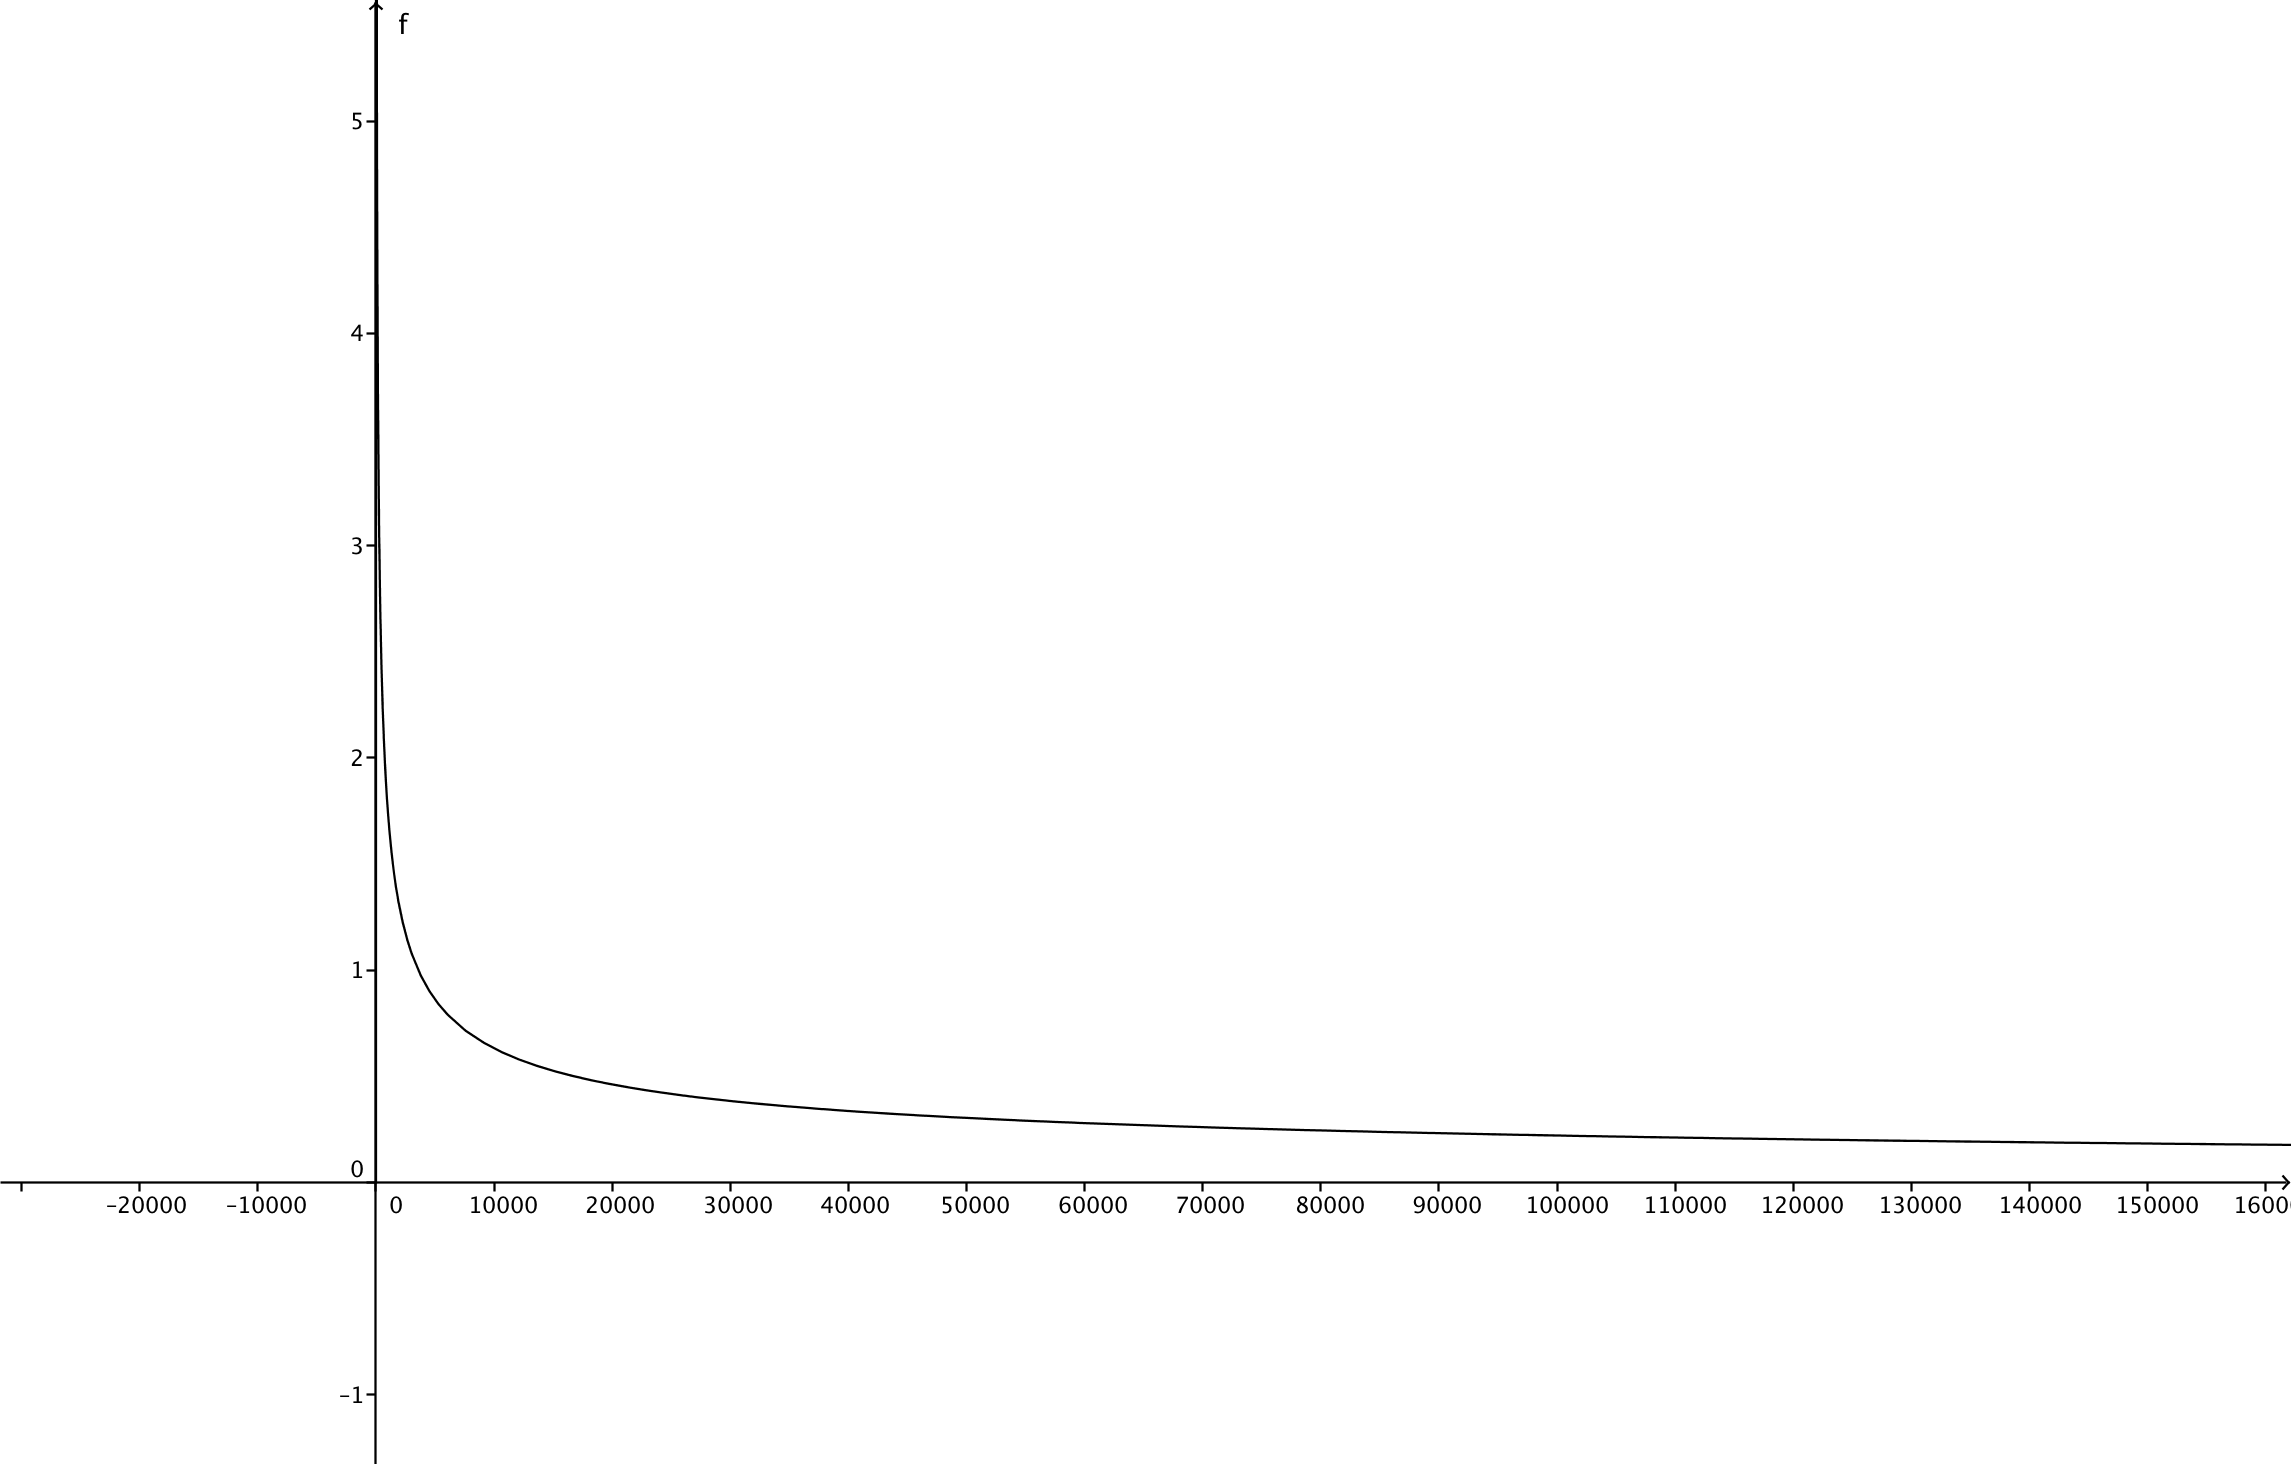
\includegraphics[scale=0.5]{OVCBound.png}
	\caption{Original VC Bound}
	\label{4-1}
\end{figure}
\begin{align}
\sqrt{\dfrac{8}{N}\ln\ParTh{\dfrac{4\ParTh{2N}^{d_{\text{vc}}}}{\delta}}}=\sqrt{\dfrac{8}{10000}\ln\ParTh{\dfrac{4\ParTh{20000}^{50}}{0.05}}}\approx0.63217
\end{align}
\item Variant VC bound:
\begin{figure}[h]
	\centering
	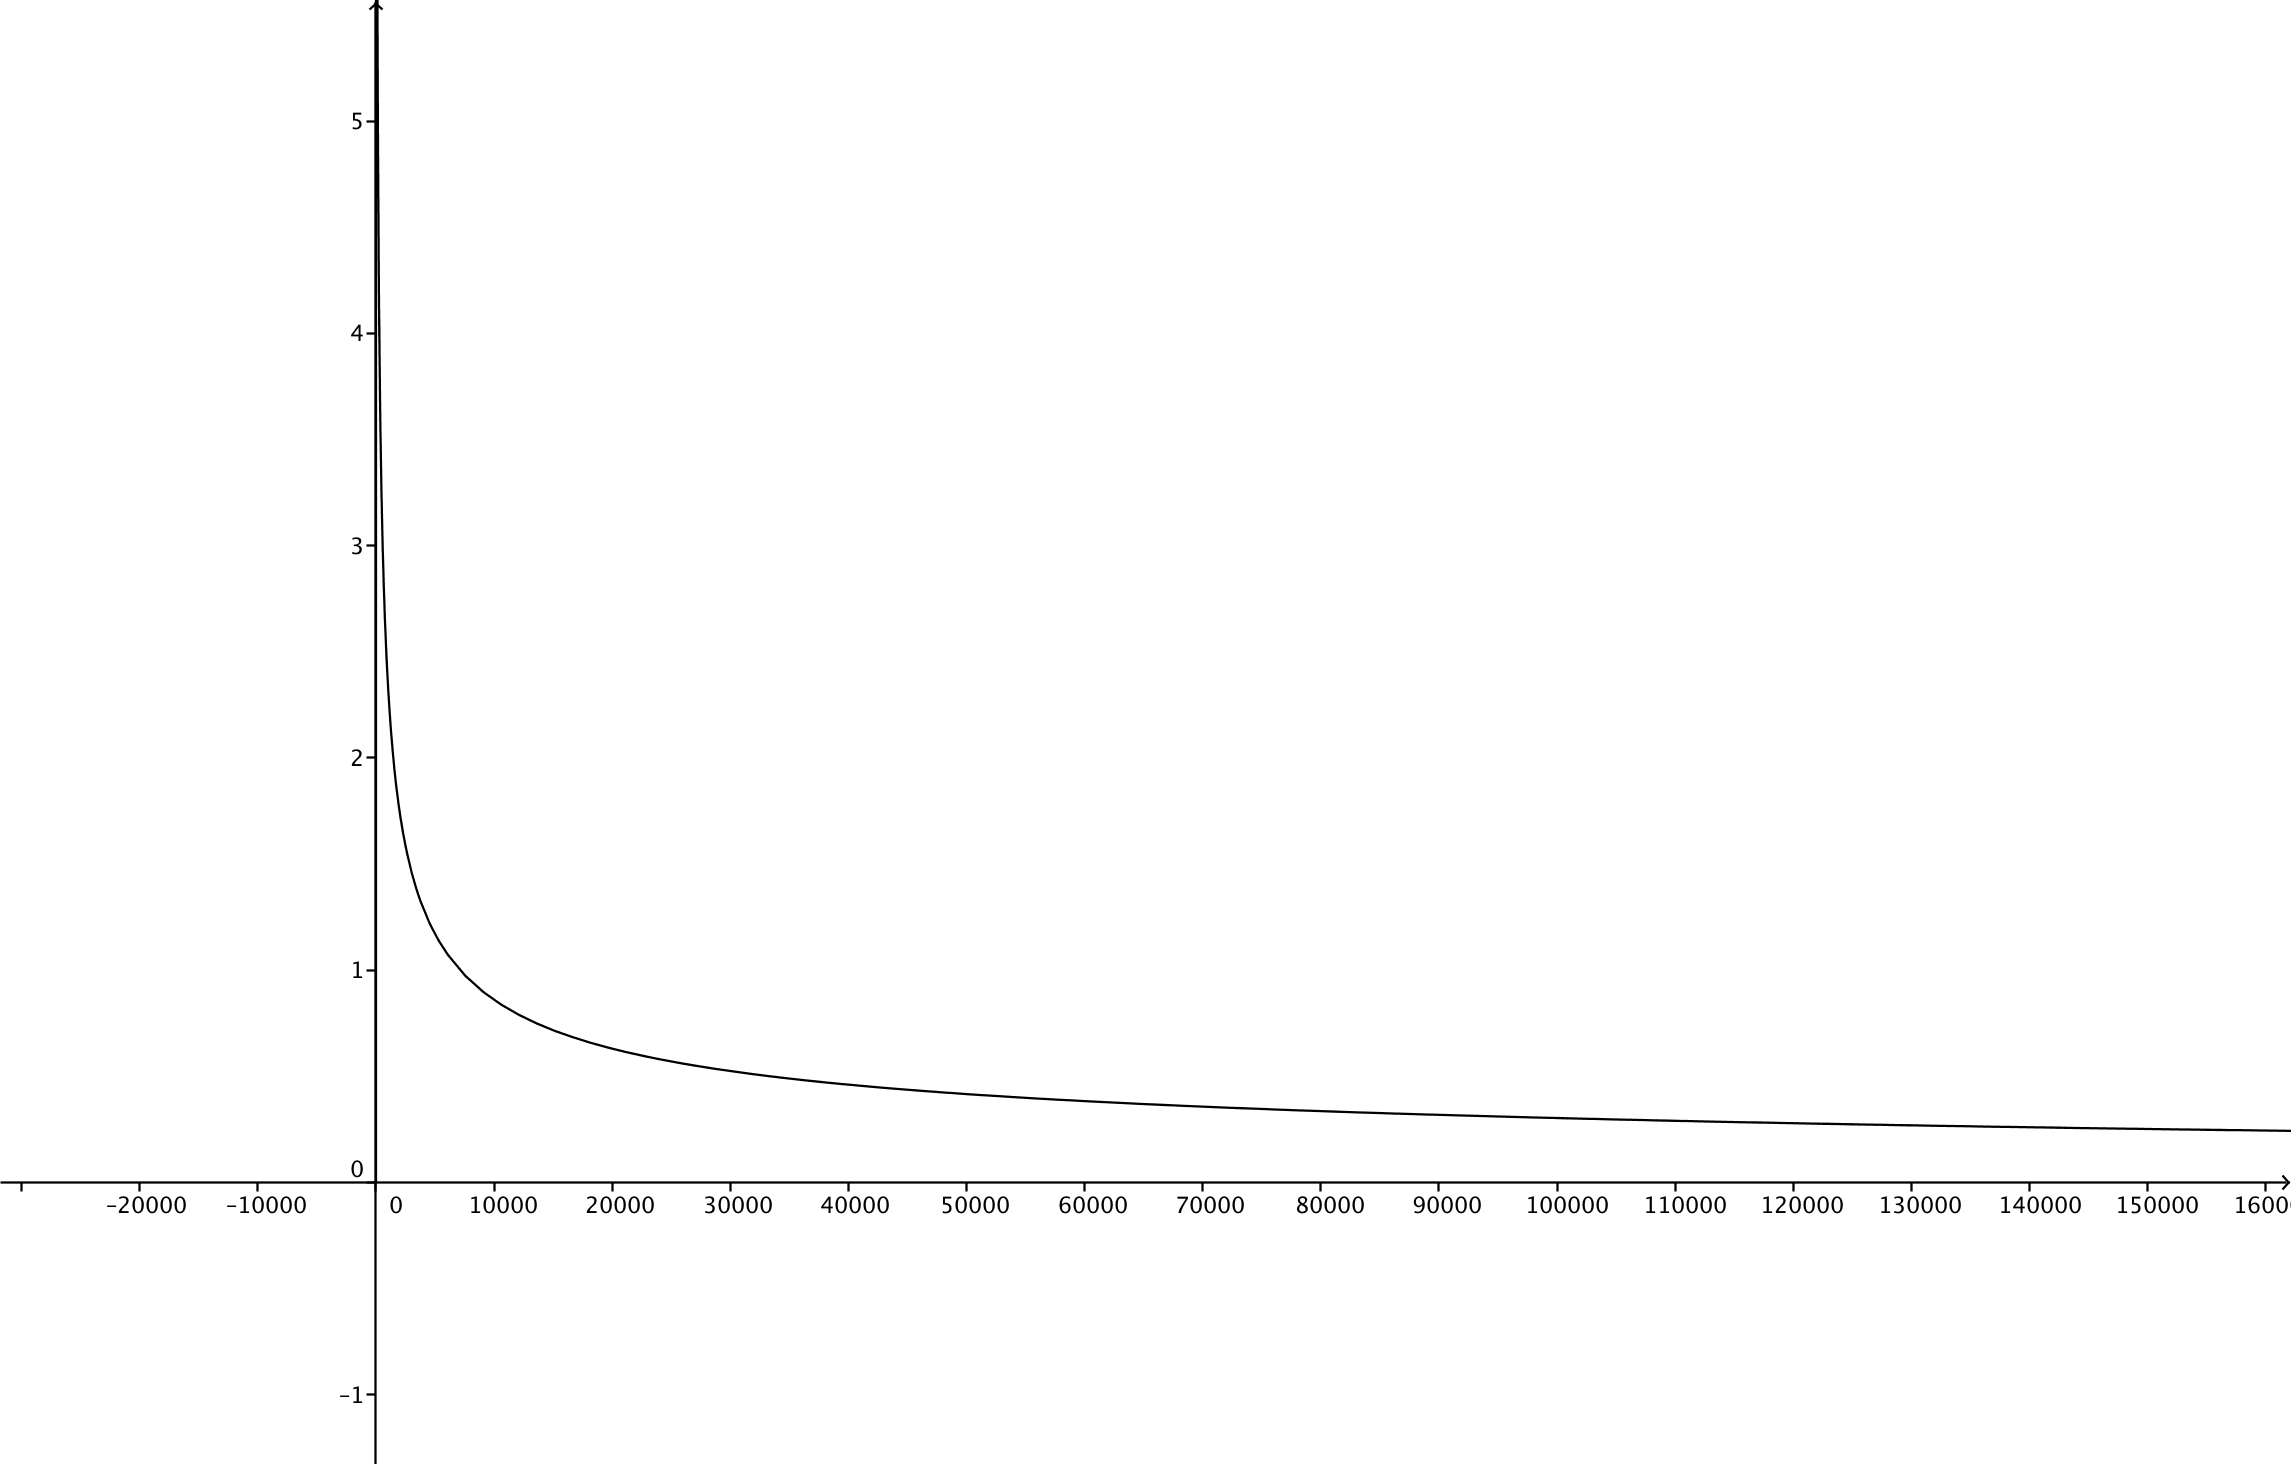
\includegraphics[scale=0.5]{VVCBound.png}
	\caption{Variant VC bound}
	\label{4-2}
\end{figure}
\begin{align}
	\sqrt{\dfrac{16}{N}\ln\ParTh{\dfrac{2\ParTh{N}^{d_{\text{vc}}}}{\sqrt{\delta}}}}&=\sqrt{\dfrac{16}{10000}\ln\ParTh{\dfrac{2\ParTh{10000}^{50}}{\sqrt{0.05}}}}\approx0.86043
\end{align}
\item Rademacher Penalty Bound:
\begin{figure}[h]
	\centering
	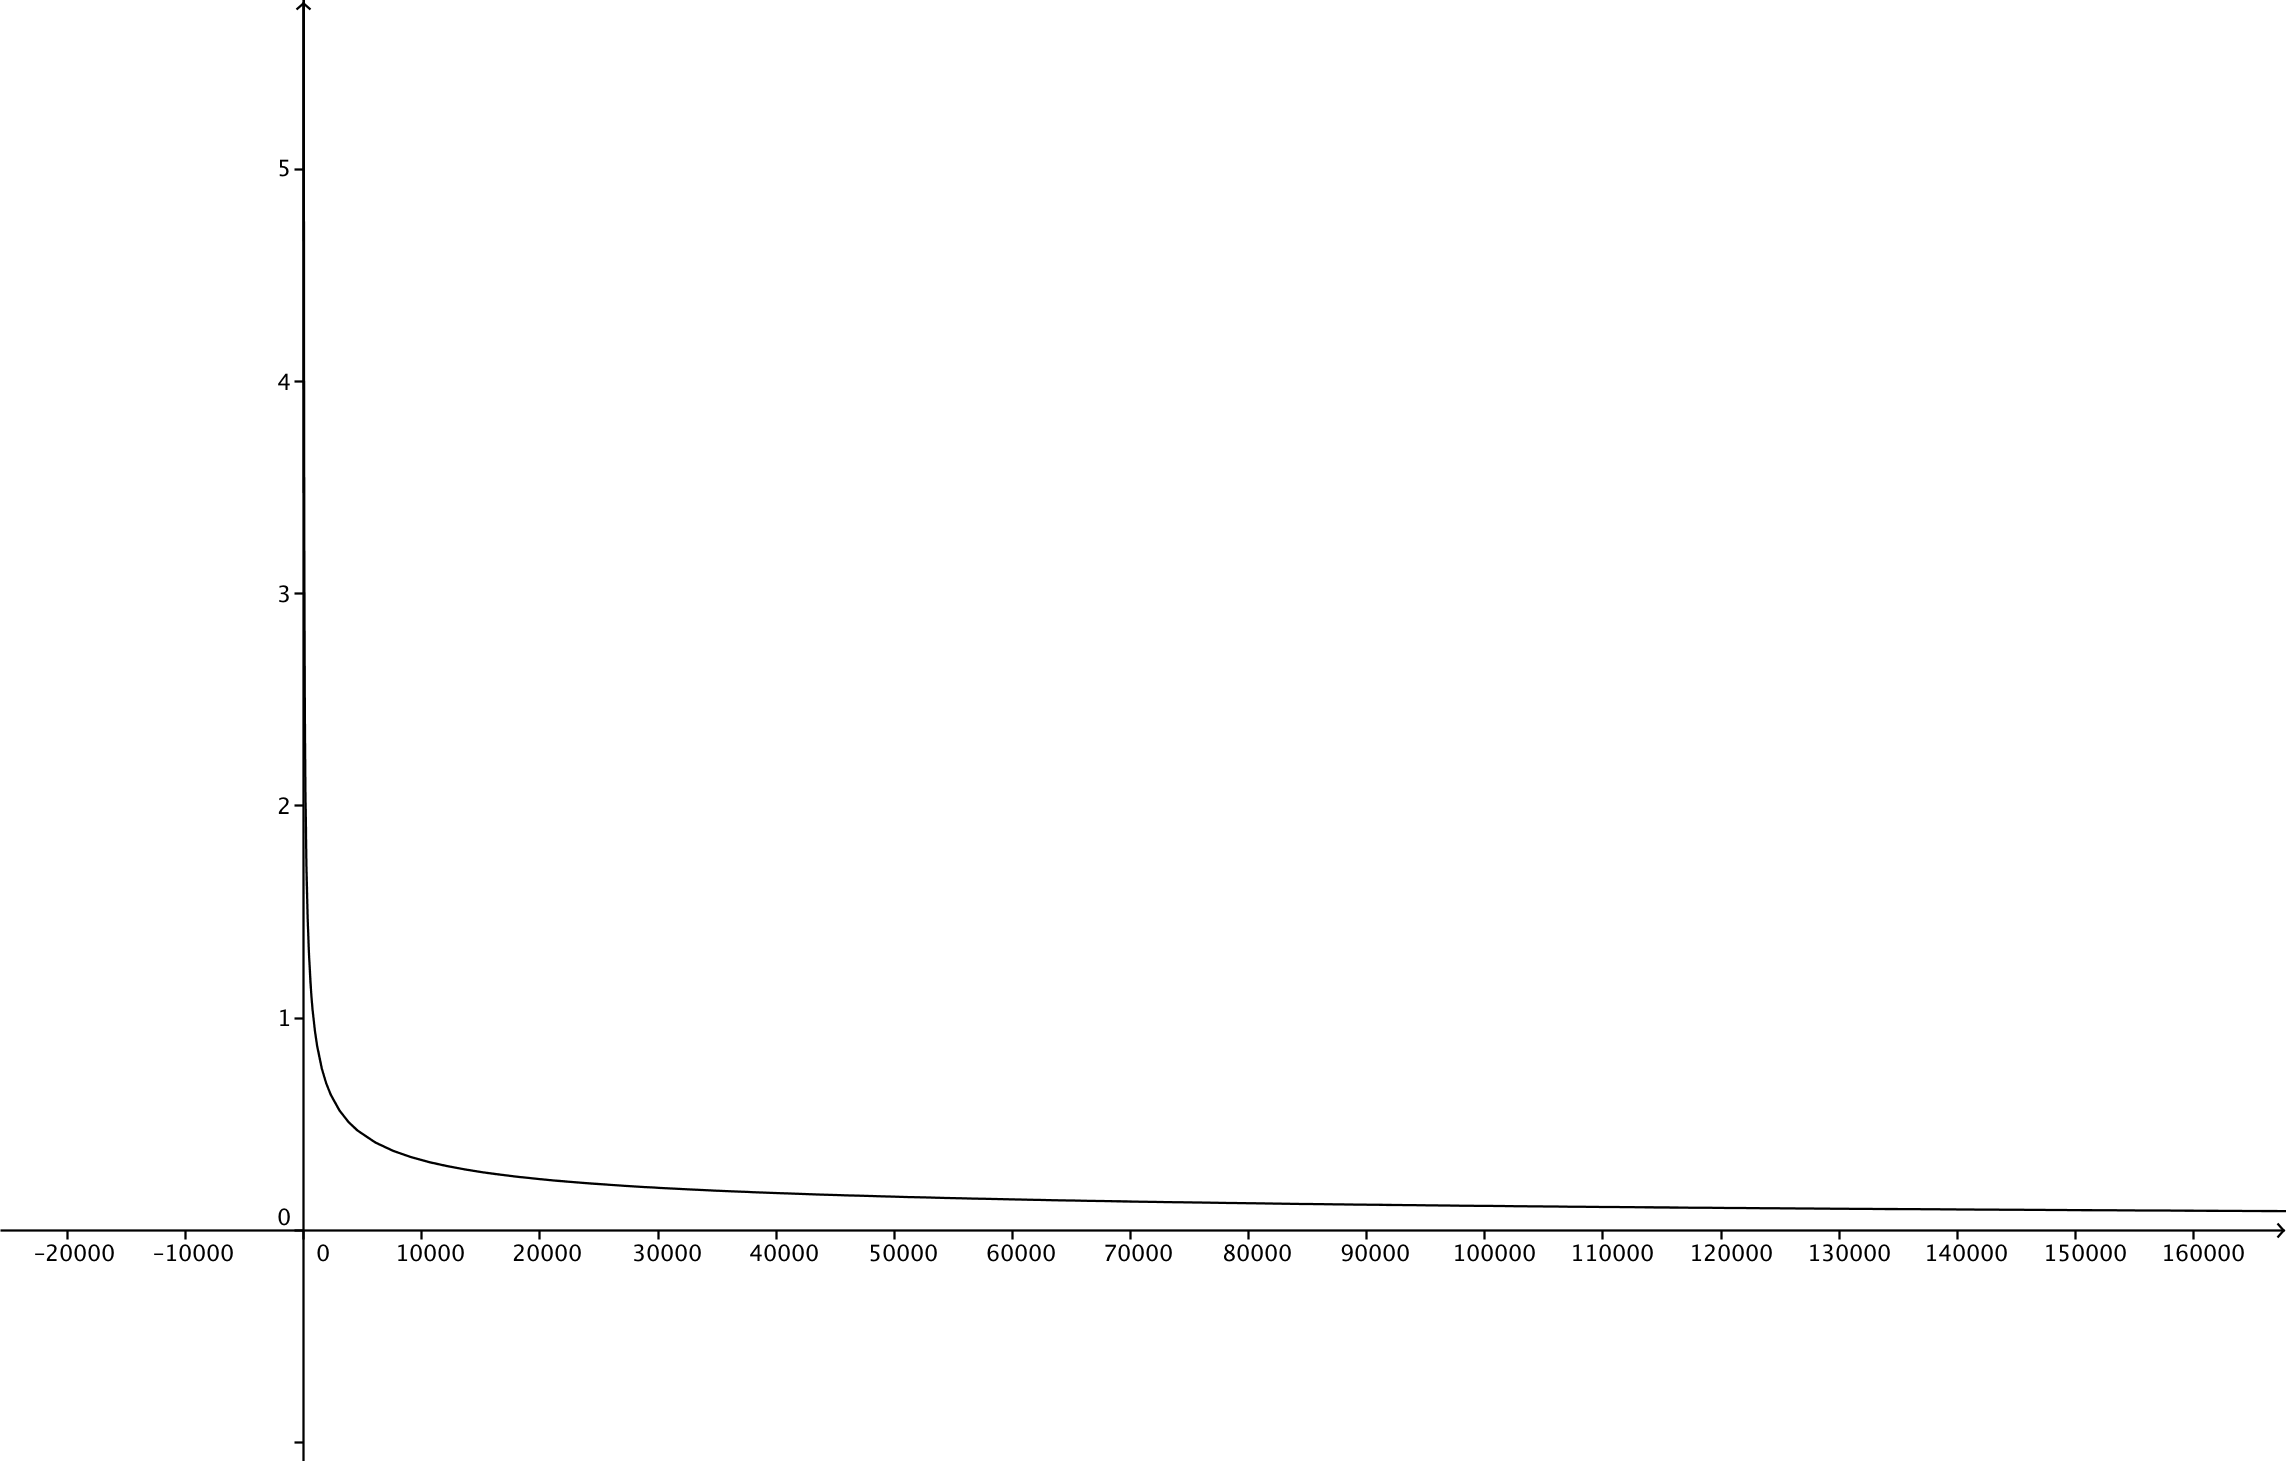
\includegraphics[scale=0.5]{RPB.png}
	\caption{Rademacher Penalty Bound}
	\label{4-3}
\end{figure}
\begin{align}
&\sqrt{\dfrac{2\ln\ParTh{{2N\ParTh{N}^{d_{\text{vc}}}}}}{N}}+\sqrt{\dfrac{2}{N}\ln\ParTh{\dfrac{1}{\delta}}}+\dfrac{1}{N}\\=&\sqrt{\dfrac{2\ln\ParTh{20000\ParTh{10000}^{50}}}{10000}}+\sqrt{\dfrac{2}{10000}\ln\ParTh{\dfrac{1}{0.05}}}+\dfrac{1}{10000}\\\approx&0.33131
\end{align}
\item Parrondo and Van den Broek:
\begin{figure}[h]
	\centering
	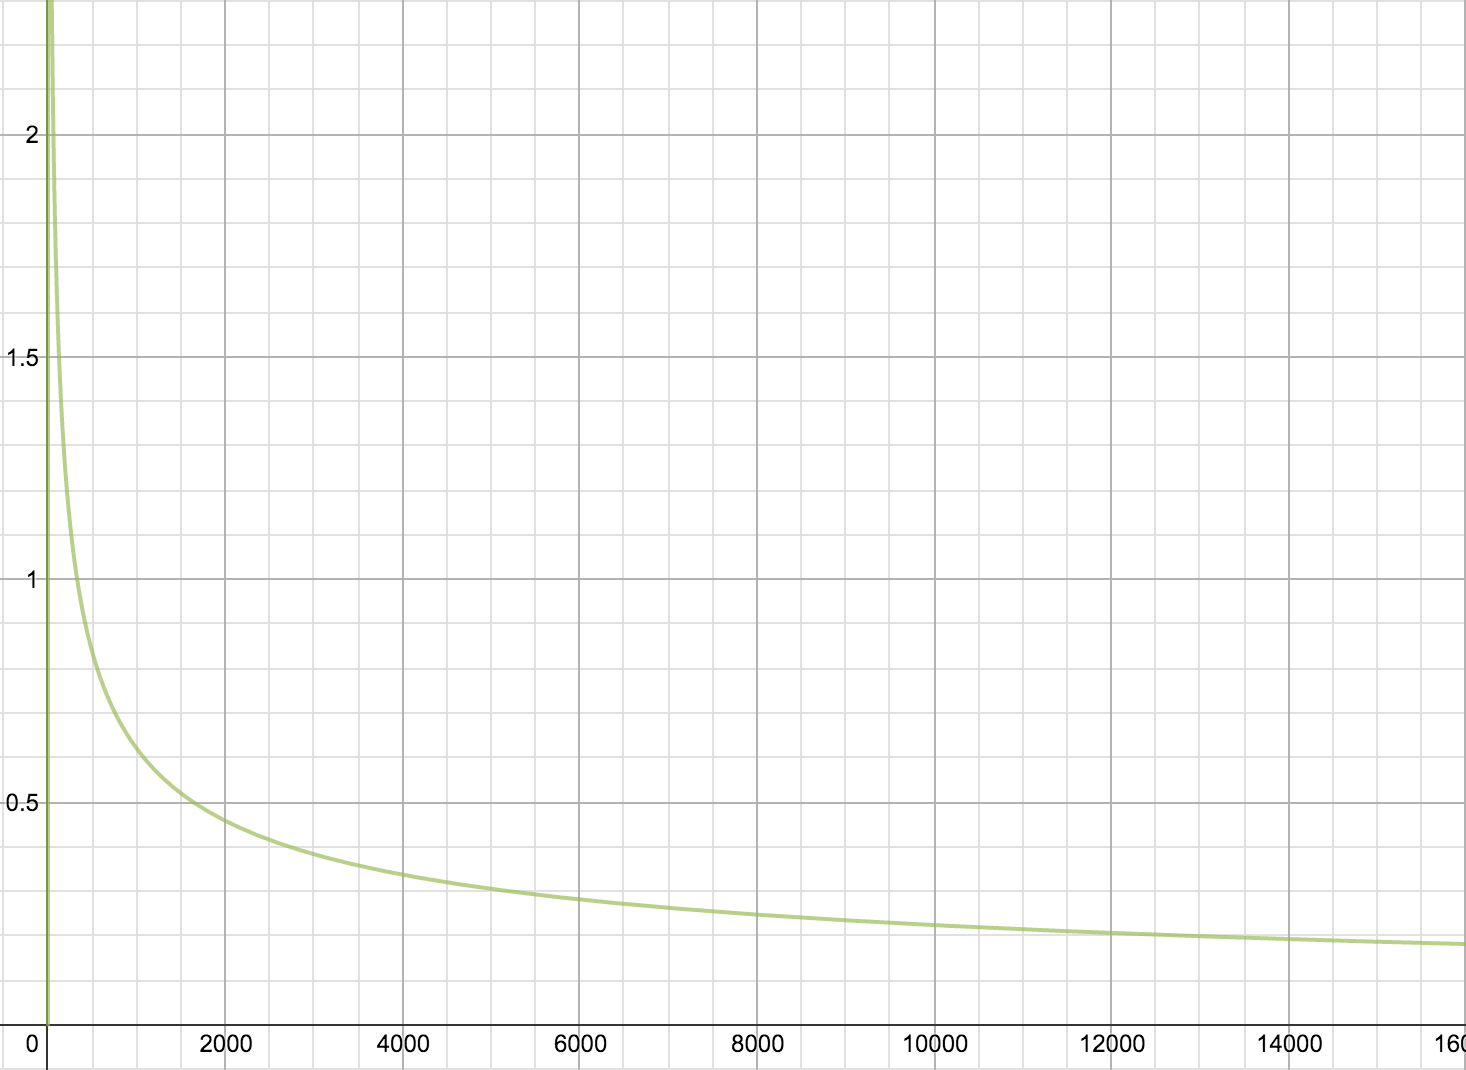
\includegraphics[scale=0.4]{PVB.png}
	\caption{Parrondo and Van den Broek}
	\label{4-4}
\end{figure}
\begin{align}
\epsilon&\leq\sqrt{\dfrac{1}{N}\ParTh{2\epsilon+\ln\ParTh{\dfrac{6\ParTh{2N}^{d_{\text{vc}}}}{\delta}}}}=\sqrt{\dfrac{1}{10000}\ParTh{2\times\epsilon+\ln\ParTh{\dfrac{6\ParTh{20000}^{50}}{0.05}}}}\\
\Rightarrow\epsilon&\leq0.22370
\end{align}
\item Devroye:
\begin{figure}[h]
	\centering
	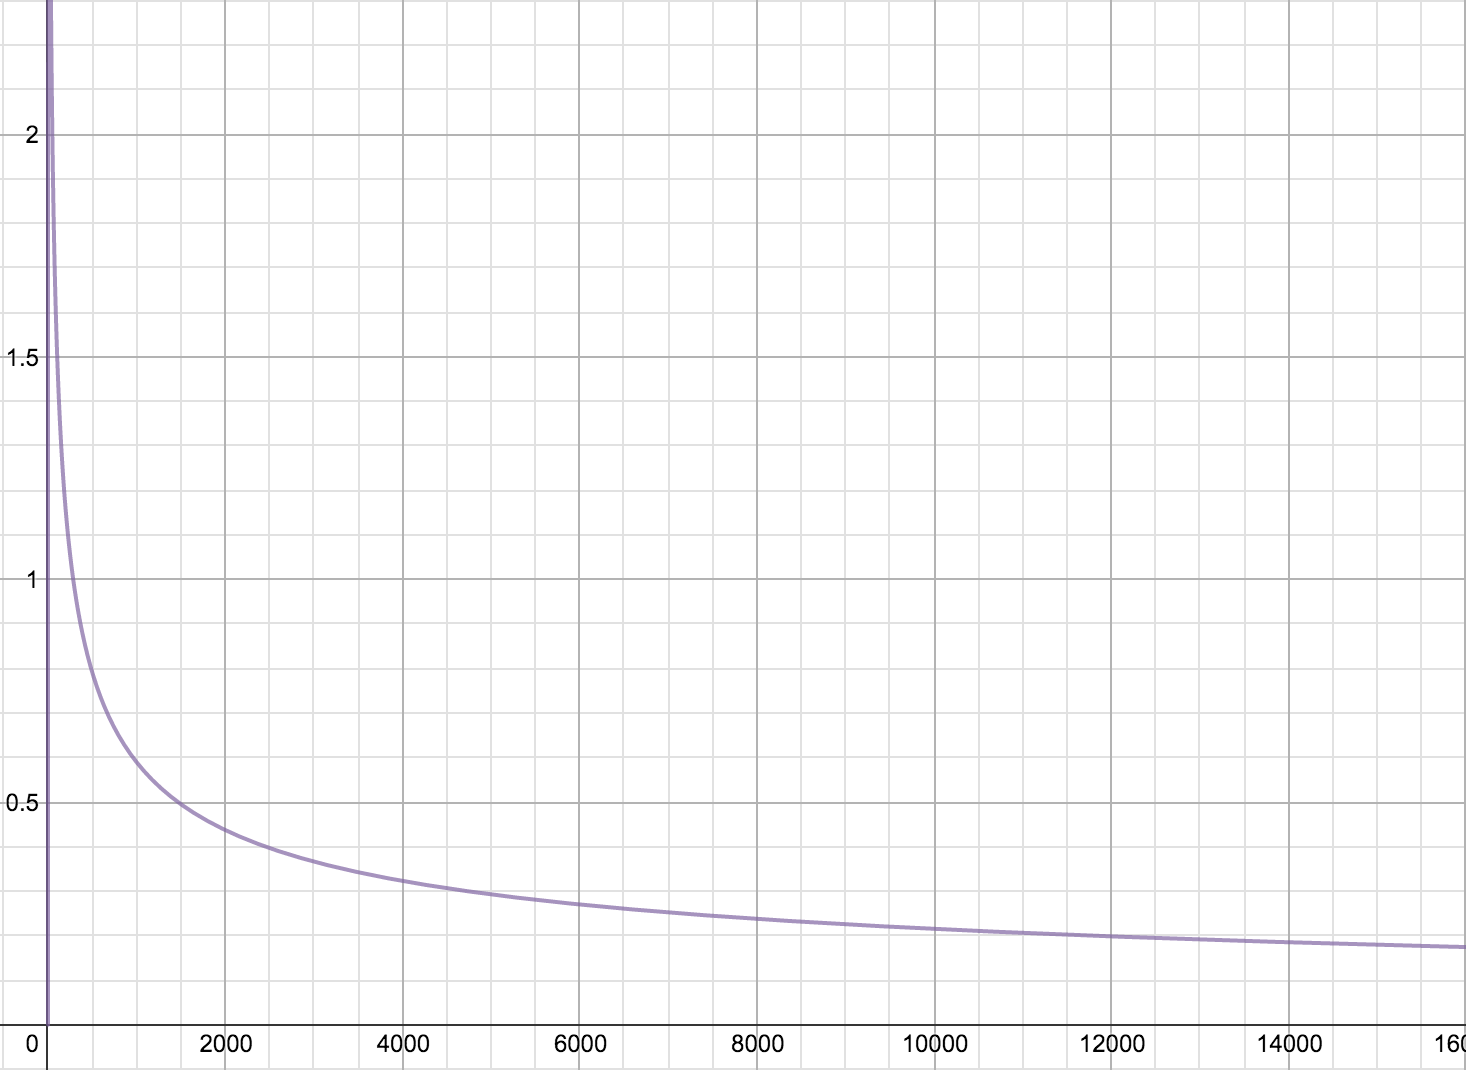
\includegraphics[scale=0.4]{D.png}
	\caption{Devroye}
	\label{4-5}
\end{figure}
\begin{align}
\epsilon\leq&\sqrt{\dfrac{1}{2N}\ParTh{4\epsilon\ParTh{1+\epsilon}+\ln\ParTh{\dfrac{4\ParTh{N^2}^{d_{\text{vc}}}}{\delta}}}}\\=&\sqrt{\dfrac{1}{20000}\ParTh{4\epsilon\ParTh{1+\epsilon}+\ln\ParTh{\dfrac{4\ParTh{{10000}^2}^{50}}{0.05}}}}\\
\Rightarrow\epsilon\leq&0.21523
\end{align}
\end{enumerate}
So the tightest bound is Devroye.

\QEDB

\horrule{0.5pt}

\subsection*{Problem 5}

Let $m_{\mathcal{H}}\ParTh{N}=\ParTh{N}^{d_{\text{vc}}}$, so
\begin{enumerate}
\item Original VC Bound:
\begin{align}
\sqrt{\dfrac{8}{N}\ln\ParTh{\dfrac{4\ParTh{2N}^{d_{\text{vc}}}}{\delta}}}=\sqrt{\dfrac{8}{5}\ln\ParTh{\dfrac{4\ParTh{10}^{50}}{0.05}}}\approx13.828
\end{align}
\item Variant VC bound:
\begin{align}
	\sqrt{\dfrac{16}{N}\ln\ParTh{\dfrac{2\ParTh{N}^{d_{\text{vc}}}}{\sqrt{\delta}}}}&=\sqrt{\dfrac{16}{5}\ln\ParTh{\dfrac{2\ParTh{5}^{50}}{\sqrt{0.05}}}}\approx16.264
\end{align}
\item Rademacher Penalty Bound:
\begin{align}
&\sqrt{\dfrac{2\ln\ParTh{{2N\ParTh{N}^{d_{\text{vc}}}}}}{N}}+\sqrt{\dfrac{2}{N}\ln\ParTh{\dfrac{1}{\delta}}}+\dfrac{1}{N}\\=&\sqrt{\dfrac{2\ln\ParTh{10\ParTh{5}^{50}}}{5}}+\sqrt{\dfrac{2}{5}\ln\ParTh{\dfrac{1}{0.05}}}+\dfrac{1}{5}\\\approx&7.0488
\end{align}
\item Parrondo and Van den Broek:
\begin{align}
\epsilon&\leq\sqrt{\dfrac{1}{N}\ParTh{2\epsilon+\ln\ParTh{\dfrac{6\ParTh{2N}^{d_{\text{vc}}}}{\delta}}}}=\sqrt{\dfrac{1}{5}\ParTh{2\epsilon+\ln\ParTh{\dfrac{6\ParTh{10}^{50}}{0.05}}}}\\
\Rightarrow\epsilon&\leq5.1014
\end{align}
\item Devroye:
\begin{align}
\epsilon\leq&\sqrt{\dfrac{1}{2N}\ParTh{4\epsilon\ParTh{1+\epsilon}+\ln\ParTh{\dfrac{4\ParTh{N^2}^{d_{\text{vc}}}}{\delta}}}}\\=&\sqrt{\dfrac{1}{10}\ParTh{4\epsilon\ParTh{1+\epsilon}+\ln\ParTh{\dfrac{4\ParTh{{5}^2}^{50}}{0.05}}}}\\
\Rightarrow\epsilon\leq&5.5931
\end{align}
\end{enumerate}
So the tightest bound is Parrondo and Van den Broek.

\QEDB

\horrule{0.5pt}

\subsection*{Problem 6}

First, choose two point as the begin and end points, we have $\binom{N}{2}+1$ choices, where $+1$ means the situation the begin and the end are the same.

Then, inside the interval should be positive or negative, there are 2 choices. Hence, we have
\begin{align}
m_{\mathcal{H}}\ParTh{N}=2\ParTh{\binom{N}{2}+1}=N^2-N+2
\end{align}

\QEDB

\horrule{0.5pt}

\subsection*{Problem 7}

For $N=4$, we have
\begin{align}
4^2-4+2=14<16=2^4
\end{align}
so the VC dimension is $4-1=3$.

\QEDB

\horrule{0.5pt}

\subsection*{Problem 8}

It is like choose two radius in ${\left(0,~N\right]}$, so we have $\binom{N+1}{2}$ choices in polar coordinate.

But we need to add the case when $a$ and $b$ make all hypothesis $-1$, which means $b^2 - a^2 < r^2_i$, $1\leq i\leq N$, where $r_i$ is the distance from origin to hypothesis point.

Hence,
\begin{align}
m_{\mathcal{H}}\ParTh{N}=\binom{N+1}{2}+1
\end{align}

\QEDB

\horrule{0.5pt}

\subsection*{Problem 9}

\begin{comment}
The function $h_c\ParTh{x}$ is
\begin{align}
h_c\ParTh{x}=\left\{
\begin{array}{ll}
+1,&\text{condition 1}\\
-1,&\text{condition 2}
\end{array}
\right.
\end{align}
The polynomial can be rewritten as
\begin{align}
\sum_{i=0}^{D}c_ix^i=c\prod_{j=1}^{D}\ParTh{x-r_j},\text{ if not all }c_i\text{ zero},~\forall i\geq1
\end{align}
where $c,~c_i\in\mathbb{R},~\forall i$ and $r_j\in\mathbb{C}$, $\forall j$. To decide $m_{\mathcal{H}}\ParTh{D}$, consider the number of imaginary roots. According to complex conjugate root theorem, we know the number of imaginary roots is even.
\begin{enumerate}
\item If $D$ is even.
\begin{align}
2\ParTh{\sum_{i=0}^{\Divide{D}{2}}\binom{D}{2i}+1}=2\sum_{i=0}^{\Divide{D}{2}}\dfrac{D!}{\ParTh{D-2i}!\ParTh{2i}!}+2=2\times2^{D-1}+2=2^D+2
\end{align}
\item If $D$ is odd.
\begin{align}
2\ParTh{\sum_{i=0}^{\Divide{\ParTh{D-1}}{2}}\binom{D}{2i}+1}=2\sum_{i=0}^{\Divide{\ParTh{D-1}}{2}}\dfrac{D!}{\ParTh{D-2i}!\ParTh{2i}!}+2=2\times2^{D-1}+2=2^D+2
\end{align}
where $+2$ is the case $c_i$ is all zero and
\begin{align}
\binom{D}{\underbracket{2k}_{\text{even}}}&=\binom{D}{\underbracket{D-2k}_{\text{odd}}},~0\leq k\leq\Divide{\ParTh{D-1}}{2}\Rightarrow\sum_{i=0}^{\Divide{\ParTh{D-1}}{2}}\binom{D}{2i}=2^{D-1}
\end{align}
\end{enumerate}
\begin{enumerate}
\item All $c_i$ are zero:
\begin{align}
\sum_{i=0}^{D}c_ix^i=0
\end{align}
only $+1$ or $-1$.
\item $c_0$ not zero and $c_i=0$, $\forall i\geq1$.
\begin{align}
\sum_{i=0}^{D}c_ix^i=c_0>0\text{ or }\sum_{i=0}^{D}c_ix^i=c_0<0
\end{align}
\item For some $m\in\mathbb{N}$, $c_i$ not zero for $0\leq i\leq m$. And $c_i = 0$ for $i>m$.

Then the degree of the polynomial is at least $m$, we have at most
\begin{align}
2{\sum_{i=0}^{k}\binom{m}{2i}}=2\times2^{m-1}=2^m
\end{align}
where $2k\leq m\leq2k+1$.
\end{enumerate}
Combine all cases, we have
\begin{align}
2^D + 2^{D-1} + 2^{D-2} + \cdots + 2^1 + 1 = 2^{D+1}-1
\end{align}
Consider
\begin{align}
	\lim\limits_{x\rightarrow\infty}\dfrac{c_nx^n}{\sum_{i=0}^{n-1}c_ix^i}
\end{align}
where $c_i\in\mathbb{R}$, $\forall i$. Apply L'Hospital rule for this formula, we have
\begin{align}
	\lim\limits_{x\rightarrow\infty}\dfrac{c_nx^n}{\sum_{i=0}^{n-1}c_ix^i}=\lim\limits_{x\rightarrow\infty}\dfrac{c_n}{c_{n-1}}x\rightarrow\infty,\text{ for }c_{n-1}\neq0
\end{align}
Now we have $D+1$ coefficients to decide how $h_c$ is. If $c_m\neq0$ and $c_k=0$, $\forall D\geq k>m\geq 0$, then $h_c=\text{sign}\ParTh{c_m}$ as $x\rightarrow\infty$ due to the conclusion above. With this, we know that the VC dimension is $D+1$ since we have $D+1$ degree of freedom.
\end{comment}
For $\sum_{i=0}^{D}c_ix^i$, we have $D$ different roots at most, separated $\mathbb{R}$ ($x$-axis) into $D+1$ sections; or no root in $\mathbb{R}$, which makes $h_c$ to be $+1$ or $-1$, $\forall x$.

The number of roots (from $0$ to $D$) forms different result in $\CBrackets{+1,~-1}^{D+1}$, like all $+1$ or $\SBrackets{+1,~-1,~+1,\ldots},\cdots$, which has at most $2^{D+1}$ choices. So the VC dimension is $D+1$.

\QEDB

\horrule{0.5pt}

\subsection*{Problem 10}

The VC dimension of simplified decision tree is equal to the number of hyper-rectangular regions, where each region returns the same $\BF{v}$.

$d$-dimension space has $2^d$ independent hyper-rectangular regions separated by $d$ lines since each dimension in $\mathbb{R}^d$ has two choices $0$ or $1$. This can shatter at most $2^d$ vectors. So the VC dimension is $2^d$.

For example, we can have $2^d$ points $\BF{x}_1$, $\BF{x}_2$,$\ldots$, $\BF{x}_{2^d}$ are different combination of $\CBrackets{-1,+1}^d$. Choose $\BF{t}=\CBrackets{0,0,\ldots,0}$, we can put each $\BF{x}_i$ in different hyper-rectangular. If $\BF{S}_i\in\BF{S}$, then $h_{\BF{t},\BF{S}}=1$, else $-1$. Hence the $2^d$ points can be shattered by choosing different collection $\BF{S}$.

If there are $2^d + 1$ points, then there are at least two points in the same hyper-rectangular region. These two points have same label no matter what $\BF{S}$ is, so the hypothesis cannot shatter $2^d+1$ points.

\QEDB

\horrule{0.5pt}

\subsection*{Problem 11}

\begin{comment}
W.L.O.G. we choose $\text{sign}\ParTh{0}=-1$.
\begin{enumerate}
	\item $h_a\ParTh{x}=-1$
	\begin{align}
	1\leq\ParTh{\alpha x\mod{4}}\leq3\Rightarrow1+4k\leq\alpha x\leq3+4k,~k\in\mathbb{Z}
	\end{align}
	\item $h_a\ParTh{x}=+1$
	\begin{align}
	0\leq\ParTh{\alpha x\mod{4}}<1&\text{ or }3<\ParTh{\alpha x\mod{4}}<4\\
	\Rightarrow4k\leq\alpha x<1+4k&\text{ or }3+4k\leq\alpha x<4+4k,~k\in\mathbb{Z}
	\end{align}
\end{enumerate}
\end{comment}
If there are $N$ point on $\mathbb{R}$, from $1^{\text{st}}$ point to $N^{\text{th}}$ point, put the $i^{\text{th}}$ point on $4^{i}$. For $1\leq k\leq2^N$, using
\begin{align}
1+\frac{1}{2}\ParTh{\frac{2k-2}{2^{N+1}}} < \alpha_k < 1+\frac{1}{2}\ParTh{\frac{2k-1}{2^{N+1}}}
\end{align}
those $\alpha_k$ can build all $\CBrackets{+1,-1}^N$ combinations, so this triangle wave hypothesis can shatter any $N$. Hence the VC dimension is $\infty$.

\QEDB

\horrule{0.5pt}

\subsection*{Problem 12}

%\begin{enumerate}
\begin{comment}
\item By definition, $m_{\mathcal{H}}\ParTh{d_vc}=2^{d_{vc}}$. Now $N\geq d_{vc}$, so $m_{\mathcal{H}}\ParTh{N}\geq2^{d_{vc}}$, which means this is not certainly an upper bound.
\item $\sqrt{N^{d_{vc}}}=N^{\Divide{d_{vc}}{2}}<N^{d_{vc}}$, which is not certainly an upper bound.
\item Since $N>\Floor{\Divide{N}{2}}$, we have $m_{\mathcal{H}}\ParTh{N}>m_{\mathcal{H}}\ParTh{\Floor{\Divide{N}{2}}}$.
\item
\end{comment}
Suppose $\min_{1\leq i\leq N-1}2^im_{\mathcal{H}}\ParTh{N-i}$ is not an upper bound.

Since $m_{\mathcal{H}}\ParTh{N}>m_{\mathcal{H}}\ParTh{m}$, $\forall m<N$. So we must have $m_{\mathcal{H}}\ParTh{N}>\min_{1\leq i\leq N-1}2^im_{\mathcal{H}}\ParTh{N-i}$. Let $i=k$ satisfies the minimum condition. Consider following cases.
\begin{enumerate}
\item $N-k< d_{vc}$.

Then we have
\begin{align}
\min_{1\leq i\leq N-1}2^im_{\mathcal{H}}\ParTh{N-i}=2^k\times2^{N-k}=2^N>m_{\mathcal{H}}\ParTh{N}
\end{align}
which is a contradiction.
\item $N-k\geq d_{vc}$.

Then we have
\begin{align}
\min_{1\leq i\leq N-1}2^im_{\mathcal{H}}\ParTh{N-i}=2^km_{\mathcal{H}}\ParTh{N-k}<m_{\mathcal{H}}\ParTh{N}<2^N
\end{align}
This is impossible since $m_{\mathcal{H}}\ParTh{d_{vc}}=2^{d_{vc}}\Rightarrow2m_{\mathcal{H}}\ParTh{d_{vc}}=2^{d_{vc}+1}>m_{\mathcal{H}}\ParTh{d_{vc}+1}$. So $2^km_{\mathcal{H}}\ParTh{N-k}>m_{\mathcal{H}}\ParTh{N}$, which leads to a contradiction.
\begin{comment}
Since $1\leq i\leq N-1$ and this holds for $N\geq d_{vc}$ by assumption. Let $N=d_{vc}+2$, we have $k=1$, then
\begin{align}
2^{d_{vc}}&<m_{\mathcal{H}}\ParTh{d_{vc}+1}<2^{d_{vc}+1}\\
\Rightarrow2^{d_{vc}+1}&<2m_{\mathcal{H}}\ParTh{d_{vc}+1}<m_{\mathcal{H}}\ParTh{d_{vc}+2}<2^{d_{vc}+2}
\end{align}
\end{comment}
\end{enumerate}
Thus, $\min_{1\leq i\leq N-1}2^im_{\mathcal{H}}\ParTh{N-i}$ is an upper bound.
%\end{enumerate}

\QEDB

\horrule{0.5pt}

\subsection*{Problem 13}

%\begin{enumerate}
\begin{comment}
\item $m_{\mathcal{H}}\ParTh{N}=N^2-N+2$ is the growth function of Problem 6.
\item $m_{\mathcal{H}}\ParTh{N}=2^N$ is the growth function of convex set.
\item $m_{\mathcal{H}}\ParTh{N}=N$ is the growth function of positive rays plus all positive case.
\item
\end{comment}
$m_{\mathcal{H}}\ParTh{N}=2^{\Floor{\sqrt{N}}}$ cannot be a growth function.

If there is no break point, the growth function should be $2^N$; if there is break point $k$, then the growth function is bounded by $\sum_{i=0}^{k-1}\binom{N}{i}$ if $k\geq 2$.

The break point is 2 since $2^{\Floor{\sqrt{2}}}=2^1<2^2$. Consider $N=25$, we have
\begin{align}
2^{\Floor{\sqrt{25}}}=2^5=32>\binom{25}{0}+\binom{25}{1}=26
\end{align}
Hence this is not a growth function.
\begin{comment}
Since $m_{\mathcal{H}}\ParTh{N^2}\leq2^{N^2}$, and
\begin{align}
m_{\mathcal{H}}\ParTh{N^2}=m_{\mathcal{H}}\ParTh{N^2+1}=\cdots=m_{\mathcal{H}}\ParTh{\ParTh{N+1}^2-1}\Rightarrow m_{\mathcal{H}}\ParTh{\ParTh{N+1}^2-1}\leq2^{N^2}
\end{align}
which violates the definition of growth function.
\end{comment}
%\end{enumerate}

\QEDB

\horrule{0.5pt}

\subsection*{Problem 14}

The smallest case of $\bigcap^K_{k=1}\mathcal{H}_k=\CBrackets{0}$, so $d_{vc}\ParTh{\CBrackets{0}}=0$.

The biggest intersection is the smallest set of $\mathcal{H}_i$, $1\leq i\leq k$, which is
\begin{align}
\CBrackets{0}\subseteq{\bigcap^K_{k=1}\mathcal{H}_k}\subseteq\min_{1\leq k\leq K}\CBrackets{{\mathcal{H}_k}}
\end{align}
Suppose $A\subseteq B$, then we have $d_{vc}\ParTh{A}\leq d_{vc}\ParTh{B}$ since if hypothesis set is greater than or equal, the VC dimension cannot be smaller.

So the upper bound of $d_{vc}\ParTh{\bigcap^K_{k=1}\mathcal{H}_k}$ is $\min_{1\leq k\leq K}\CBrackets{d_{vc}\ParTh{\mathcal{H}_k}}$. Hence
\begin{align}
0\leq d_{vc}\ParTh{\bigcap^K_{k=1}\mathcal{H}_k}\leq\min_{1\leq k\leq K}\CBrackets{d_{vc}\ParTh{\mathcal{H}_k}}
\end{align}

\QEDB

\horrule{0.5pt}

\subsection*{Problem 15}

The smallest union is the biggest set of $\mathcal{H}_i$, $1\leq i\leq k$. So the lower bound of $d_{vc}\ParTh{\bigcup^K_{k=1}\mathcal{H}_k}$ is $\max_{1\leq k\leq K}\CBrackets{d_{vc}\ParTh{\mathcal{H}_k}}$.

\underline{Claim}: $d_{vc}\ParTh{\mathcal{H}_1\cup\mathcal{H}_2}\leq d_{vc}\ParTh{\mathcal{H}_1}+d_{vc}\ParTh{\mathcal{H}_2}+1$.

\underline{Proof of claim}:

Define $d_{vc}\ParTh{\mathcal{H}_1}=d_1$, $d_{vc}\ParTh{\mathcal{H}_2}=d_2$. The number can be classified using $\mathcal{H}_1\cup\mathcal{H}_2$ is at most  the
number of classifications using $\mathcal{H}_1$ plus the number of classifications using $\mathcal{H}_2$. So
\begin{align}
m_{\mathcal{H}_1\cup\mathcal{H}_2}\ParTh{N}\leq m_{\mathcal{H}_1}\ParTh{N}+m_{\mathcal{H}_2}\ParTh{N}
\end{align}
Since $B\ParTh{N,K}\leq\sum_{i=0}^{d}\binom{N}{i}$ ($d=K-1$), we have
%By $\text{Sauer-Shelah Lemma}^{[2]}$, we have
\begin{align}
m_{\mathcal{H}_1\cup\mathcal{H}_2}\ParTh{N}\leq\sum_{i=0}^{d_1}\binom{N}{i}+\sum_{i=0}^{d_2}\binom{N}{i}
\end{align}
Then
\begin{align}
m_{\mathcal{H}_1\cup\mathcal{H}_2}\ParTh{N}\leq\sum_{i=0}^{d_1}\binom{N}{i}+\sum_{i=0}^{d_2}\binom{N}{N-i}=\sum_{i=0}^{d_1}\binom{N}{i}+\sum_{i=N-d_2}^{N}\binom{N}{i}
\end{align}
Now, if $N - d_2 > d_1 + 1$, that is $N \geq d_1 + d_2 + 2$.
\begin{align}
m_{\mathcal{H}_1\cup\mathcal{H}_2}\ParTh{N}&\leq\sum_{i=0}^{N}\binom{N}{i}-\binom{N}{d_1+1}=2^N-\binom{N}{d_1+1}<2^N\\
\Rightarrow m_{\mathcal{H}_1\cup\mathcal{H}_2}\ParTh{N}&<2^{d_1+d_2+2}\\
\Rightarrow m_{\mathcal{H}_1\cup\mathcal{H}_2}\ParTh{N}&\leq2^{d_1+d_2+1}
\end{align}
If $N-d_2\leq d_1+1$, then we have $N\leq d_1+d_2+1$ and
\begin{align}
\underbrace{m_{\mathcal{H}_1\cup\mathcal{H}_2}\ParTh{N}\leq2^N}_{\text{holds for all }m_{\mathcal{H}}\ParTh{N}}\leq2^{d_1+d_2+1}
\end{align}
Hence, $d_{vc}\ParTh{\mathcal{H}_1\cup\mathcal{H}_2}\leq d_1+d_2+1$.

From the equation above, we have
\begin{align}
\max_{1\leq k\leq K}\CBrackets{d_{vc}\ParTh{\mathcal{H}_k}}\leq d_{vc}\ParTh{\bigcup^K_{k=1}\mathcal{H}_k}\leq \ParTh{K-1}+\sum_{i=1}^{K}d_{vc}\ParTh{\mathcal{H}_i}
\end{align}

\QEDB

\horrule{0.5pt}

\subsection*{Problem 16}

If $s = +1$, consider following cases.
\begin{enumerate}
\item $h_{s,\theta}\ParTh{x}=-1$ as $\text{sign}\ParTh{x}=+1\Rightarrow 0<x\leq\theta\leq+1$.
\item $h_{s,\theta}\ParTh{x}=+1$ as $\text{sign}\ParTh{x}=-1\Rightarrow -1\leq\theta\leq x\leq0$.
\end{enumerate}
%This can be rewritten as $x<\AbsVal{\theta}$.
\begin{comment}
\begin{enumerate}
\item $h_{s,\theta}\ParTh{x}=-1$ as $\text{sign}\ParTh{x}=+1$.

Since $\mathbb{P}\ParTh{\text{sign}\ParTh{x}=+1}=\Divide{1}{2}$ and $\text{sign}\ParTh{x}=+1\Rightarrow x\in\left(0,+1\right]$. Then \begin{align}
\mathbb{P}\ParTh{\left. h_{s,\theta}\ParTh{x}=-1 \middle| x\in\left(0,+1\right] \right.}=\mathbb{P}\ParTh{\left.\theta\geq x\middle| x\in\left(0,+1\right] \right.}=\underbrace{\dfrac{1}{2}}_{\theta>0}\times\underbrace{\dfrac{\theta}{2}}_{0<x\leq\theta}=\dfrac{\theta}{4}
\end{align}
\item $h_{s,\theta}\ParTh{x}=+1$ as $\text{sign}\ParTh{x}=-1$.

Since $\mathbb{P}\ParTh{\text{sign}\ParTh{x}=-1}=\Divide{1}{2}$ and $\text{sign}\ParTh{x}=-1\Rightarrow x\in\SBrackets{-1,0}$. Then \begin{align}
\mathbb{P}\ParTh{\left. h_{s,\theta}\ParTh{x}=+1\middle|x\in\SBrackets{-1,0}\right.}=\mathbb{P}\ParTh{\left. \theta< x\middle|x\in\SBrackets{-1,0}\right.}=\underbrace{\dfrac{1}{2}}_{\theta<0}\times\underbrace{\dfrac{\AbsVal{\theta}}{2}}_{-1\leq\theta<x}=\dfrac{\AbsVal{\theta}}{4}
\end{align}
\end{enumerate}
\end{comment}
So we have $\mathbb{P}\ParTh{h_{+1,\theta}\ParTh{x}\neq\text{sign}\ParTh{x}}=\Divide{\AbsVal{\theta}}{2}$, then $E_{out}$ is
\begin{align}
E_{out}=\underbrace{ 0.2 \times \ParTh{1-\dfrac{\AbsVal{\theta}}{2}} }_{\text{fliped}}+\underbrace{ 0.8 \times \dfrac{\AbsVal{\theta}}{2} }_{\text{no fliped}}=0.2+0.3\AbsVal{\theta}
\end{align}
Similarly, if $s=-1$, , then $E_{out}$ is
\begin{align}
E_{out}=\underbrace{ 0.2 \times \dfrac{\AbsVal{\theta}}{2} }_{\text{fliped}}+\underbrace{ 0.8 \times \ParTh{1-\dfrac{\AbsVal{\theta}}{2}} }_{\text{no fliped}}=0.8-0.3\AbsVal{\theta}
\end{align}
Combine two cases, we have
\begin{align}
E_{out}=0.5+0.3s\ParTh{\AbsVal{\theta}-1}
\end{align}

\QEDB

\horrule{0.5pt}

\newpage
\subsection*{Problem 17}

The average $E_{in}=0.17123$.
\begin{figure}[h]
	\centering
	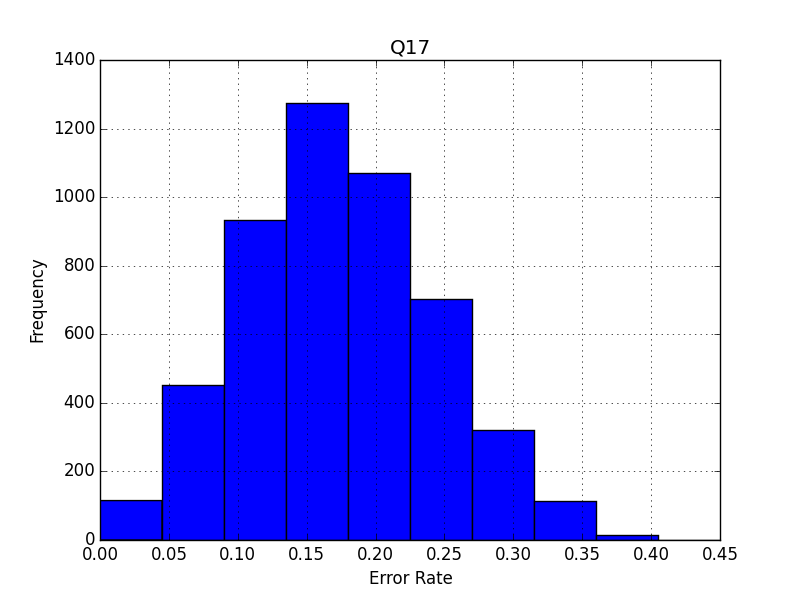
\includegraphics[scale=0.3]{Q17.png}
	\caption{Q17 histogram}
	\label{Q18}
\end{figure}

\QEDB

\horrule{0.5pt}

\subsection*{Problem 18}

The average $E_{out}=0.26586$.
\begin{figure}[h]
	\centering
	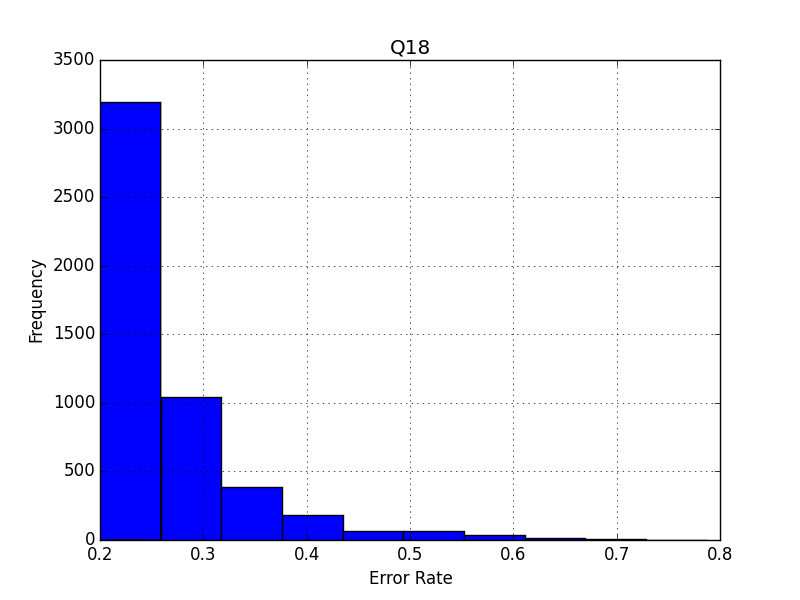
\includegraphics[scale=0.3]{Q18.png}
	\caption{Q18 histogram}
	\label{Q18}
\end{figure}

\QEDB

\horrule{0.5pt}

\subsection*{Problem 19}

The optimal decision stump is the fourth dimension. The $E_{in}=0.25000$. The optimal decision stump is the $4^{\text{th}}$ column.

\QEDB

\horrule{0.5pt}

\subsection*{Problem 20}

The $E_{out}=E_{test}=0.36000$.

\QEDB

\horrule{0.5pt}

\subsection*{Problem 21}

\begin{comment}
Prove $B\ParTh{N,k}\geq\sum_{i=0}^{k-1}\binom{N}{i}$ by induction on $N$.
\begin{enumerate}
	\item Since $N\geq k$. Suppose $N=M\geq k$ the equation holds
	\begin{align}
	B\ParTh{M,k}\geq\sum_{i=0}^{k-1}\binom{M}{i}
	\end{align}
	\item Consider $N=M+1$, we have
	\begin{align}
	B\ParTh{M,k}=B
	\end{align}
\end{enumerate}
\end{comment}
Consider any $\mathcal{H}=\CBrackets{-1,+1}^N$, with $N\geq k\geq 1$. If there are at most $k-1$ variables be $-1$. We have $m_{\mathcal{H}}\ParTh{N}=\sum_{i=0}^{k-1}\binom{N}{i}$ dichotomies with no subset of $k$ variables can be shattered.

Since $B\ParTh{N,k}$ bounds $m_{\mathcal{H}}\ParTh{N}$, we have
\begin{align}
B\ParTh{N,k}\geq\sum_{i=0}^{k-1}\binom{N}{i}
\end{align}
Combine the conclusion $B\ParTh{N,k}\leq\sum_{i=0}^{k-1}\binom{N}{i}$, which had been proved in class, we have
\begin{align}
B\ParTh{N,k}=\sum_{i=0}^{k-1}\binom{N}{i}
\end{align}

\QEDB

\horrule{0.5pt}

\section*{Reference}

\begin{enumerate}

\item[{[1]}] Lecture Notes by Hsuan-Tien LIN, Department of Computer Science and Information Engineering, National Taiwan University, Taipei 106, Taiwan.

%\item[{[2]}] Three proofs of Sauer-Shelah Lemma. (n. d. ). Retrieved Fall, 2010, from \url{http://www.cse.buffalo.edu/~hungngo/classes/2010/711/lectures/sauer.pdf}

\end{enumerate}

\end{document}